\documentclass{article}
\linespread{1.3}
\usepackage[margin=50pt]{geometry}
\usepackage{amsmath, amsthm, amssymb, amsthm, tikz, fancyhdr, float, graphicx, spverbatim, systeme}
\pagestyle{fancy}
\renewcommand{\headrulewidth}{0pt}
\newcommand{\changefont}{\fontsize{15}{15}\selectfont}

\fancypagestyle{firstpageheader}{
  \fancyhead[R]{
    \changefont
    \parbox[t]{4cm}{ % Adjust width as needed
      Michael Huang\\
      EN.555.644.81\\
      Homework 11
    }
  }
}

\begin{document}

\thispagestyle{firstpageheader}
{\Large 

\section*{15.3}
Calculate the price of a three-month European put option on a non-dividend-paying stock with a strike price of \$50 when the current stock price is \$50, the risk-free interest rate is 10\% per annum, and the volatility is 30\% per annum. \\ \\
We use the BSM forumlas, with \(S_0 = 50, K = 50, r = 0.10, \sigma = 0.30, T = \frac{3}{12} = \frac{1}{4}\):
\[
  d_1 = \frac{\ln(S_0 / K) + (r + \sigma^2 / 2)T}{\sigma \sqrt{T}}
\]
\[
  = \frac{\ln(\frac{50}{50}) + (0.10 + \frac{0.3^2}{2}) \cdot \frac{1}{4}}{0.3 \cdot \sqrt{\frac{1}{4}}}
\]
\[
  d_1 = \frac{0 + 0.03625}{0.15} = 0.2416666666
\]
and accordingly:
\[
  d_2 = d_1 - \sigma \sqrt{T}
\]
\[
  d_2 = 0.2416666666 - 0.3 \cdot \sqrt{\frac{1}{4}} = 0.2416666666 - 0.15 = 0.0916666666
\]
The price of the put is therefore
\[
  p = Ke^{-rT} N(-d_2) - S_0 N(-d_1)
\]
\[
  = 50 e^{-0.1 \cdot 0.25} N(-0.0916666666) - 50  N(-0.2416666666)
\]
looking at a standard normal cdf table and approximating: 
\[
  = 50 e^{-0.025} \cdot 0.4641 - 50 \cdot 0.4052
\]
\[
  p = 22.6320665084 - 20.26 = 2.3720665084 \approx \boxed{\textbf{\$2.37}}
\]

}
{\Large 

\section*{15.4}
What difference does it make to your calculations in Problem 15.3 if a dividend of \$1.50 is expected in two months? \\ \\
The addition of the dividend means that we have to discount the current stock price accordingly:
\[
  S_0 = 50 - 1.50e^{-0.10 \cdot \frac{2}{12}} = 50 - 1.50 e^{-\frac{1}{60}}
\]
\[
  S_0 = 50 - 1.50 \cdot 0.98347145382 = 50 - 1.47520718073 = 48.5247928193
\]
We now plug in this new value for \(S_0\), keeping the other values the same:
\[
  d_1 = \frac{\ln(S_0 / K) + (r + \sigma^2 / 2)T}{\sigma \sqrt{T}}
\]
\[
  = \frac{\ln(\frac{48.5247928193}{50}) + (0.10 + \frac{0.3^2}{2}) \cdot \frac{1}{4}}{0.3 \cdot \sqrt{\frac{1}{4}}}
\]
\[
  d_1 = \frac{-0.02994814595 + 0.03625}{0.15} = 0.04201236033
\]
and accordingly:
\[
  d_2 = d_1 - \sigma \sqrt{T}
\]
\[
  d_2 = 0.04201236033 - 0.3 \cdot \sqrt{\frac{1}{4}} = 0.04201236033 - 0.15 = -0.10798763967
\]
The price of the put is therefore
\[
  p = Ke^{-rT} N(-d_2) - S_0 N(-d_1)
\]
\[
  = 50 e^{-0.1 \cdot 0.25} N(0.10798763967) - 50  N(-0.04201236033)
\]
looking at a standard normal cdf table and approximating: 
\[
  = 50 e^{-0.025} \cdot 0.5438 - 48.5247928193 \cdot 0.4840
\]
\[
  p = 26.5186765078 - 23.4859997245 = 3.0326767833 \approx \boxed{\textbf{\$3.03}}
\]



}
{\Large 

\section*{15.9}
Assume that a non-dividend-paying stock has an expected return of \(\mu\) and a volatility of \(\sigma\). An innovative financial institution has just announced that it will trade a derivative that pays off a dollar amount equal to \(\ln S_T\) at time \(T\) where \(S_T\) denotes the values of the stock price at time \(T\).

\subsection*{(a)} 
Use risk-neutral valuation to calculate the price of the derivative at time \(t\) in term of the stock price, \(S\), at time \(t\) \\ \\
To use the risk-neutral valuation, we compute the expected value assuming that the stock's expected return is the risk-free rate \(r\), and then discount accordingly. From the lognormal property of stock prices, we know that 
\[
  \ln(S_T) \sim \phi[\ln(S_0) + (\mu - \frac{\sigma^2}{2})T, \sigma^2 T]
\]
so the risk-neutral expected value is 
\[
  \ln(S) + (r - \frac{\sigma^2}{2})(T-t)
\]
and discounting accordingly, the price of the derivative should be 
\[
  \boxed{\mathbf{[\ln(S) + (r - \frac{\sigma^2}{2})(T-t)]e^{-r(T-t)}}}
\]

\subsection*{(b)}
Confirm that your price satisfies the differential equation (15.16) \\ \\
Equation (15.16) indicates that 
\[
  \frac{\partial f}{\partial t} + r S \frac{\partial f}{\partial S} + \frac{1}{2} \sigma^2 S^2 \frac{\partial^2 f}{\partial S^2} = rf
\]
and with \(f = [\ln(S) + (r - \frac{\sigma^2}{2})(T-t)]e^{-r(T-t)}\), we can calculate the following: \\
- \(\frac{\partial f}{\partial t} = [\ln(S) + (r - \frac{\sigma^2}{2})(T-t)] \cdot re^{-r(T-t)} - [r - \frac{\sigma^2}{2}] \cdot e^{-r(T-t)} \) \\ 
- \(\frac{\partial f}{\partial S} = (\frac{1}{S} + 0)e^{-r(T-t)} = \frac{e^{-r(T-t)}}{S} \) \\
- \(\frac{\partial^2 f}{\partial S^2} = - \frac{e^{-r(T-t)}}{S^2}\) \\
So plugging this in: \\
\(
  [\ln(S) + (r - \frac{\sigma^2}{2})(T-t)] re^{-r(T-t)} - [r - \frac{\sigma^2}{2}] e^{-r(T-t)} + r S \cdot \frac{e^{-r(T-t)}}{S} + \frac{1}{2} \sigma^2 S^2 \cdot - \frac{e^{-r(T-t)}}{S^2}
\) \\
\[
  = e^{-r(T-t)}[r\ln(S) + r(r - \frac{\sigma^2}{2})(T-t) - r + \frac{\sigma^2}{2} + r - \frac{\sigma^2}{2}]
\]
\[
  = e^{-r(T-t)}[r\ln(S) + r(r - \frac{\sigma^2}{2})(T-t)]
\]
\[
  = r \cdot [\ln(S) + (r - \frac{\sigma^2}{2})(T-t)]e^{-r(T-t)}
\]
\[
  = rf
\]
exactly as we aimed to find. 

}
{\Large 

\section*{15.11}
What is the price of a European call option on a non-dividend-paying stock when the stock price is \$52, the strike price is \$50, the risk-free interest rate is 12\% per annum, the volatility is 30\% per annum, and the time to maturity is three months? \\ \\
We use the BSM forumlas, with \(S_0 = 52, K = 50, r = 0.12, \sigma = 0.30, T = \frac{3}{12} = \frac{1}{4}\):
\[
  d_1 = \frac{\ln(S_0 / K) + (r + \sigma^2 / 2)T}{\sigma \sqrt{T}}
\]
\[
  = \frac{\ln(\frac{52}{50}) + (0.12 + \frac{0.3^2}{2}) \cdot \frac{1}{4}}{0.3 \cdot \sqrt{\frac{1}{4}}}
\]
\[
  d_1 = \frac{0.03922071315 + 0.04125}{0.15} = \frac{0.08047071315}{0.15} = 0.536471421
\]
and accordingly:
\[
  d_2 = d_1 - \sigma \sqrt{T}
\]
\[
  d_2 = 0.536471421 - 0.3 \cdot \sqrt{\frac{1}{4}} = 0.536471421 - 0.15 = 0.386471421
\]
The price of the call is therefore
\[
  c = S_0 N(d_1) - Ke^{-rT} N(d_2)
\]
\[
  = 52 N(0.536471421) - 50 e^{-0.12 \cdot 0.25} N(0.386471421)
\]
looking at a standard normal cdf table and approximating: 
\[
  = 52 \cdot 0.7054 - 50 e^{-0.03} \cdot 0.6517
\]
\[
  c = 36.6808 - 31.6219677104 = 5.0588322896 \approx \boxed{\textbf{\$5.06}}
\]

}
{\Large 

\section*{15.13}
Consider an American call option on a stock. The stock price is \$70, the time to maturity is eight months, the risk-free rate of interest is 10\% per annum, the exercise price is \$65, and the volatility is 32\%. A dividend of \$1 is expected after three months and again after six months. Show that it can never be optimal to exercise the option on either of the two dividend dates. Use DerivaGem to calculate the price of the option. \\ \\
For the American call option, we have \(S_0 = 70, T = \frac{8}{12} = \frac{2}{3}, r = 0.10, K = 65, \sigma = 0.32, D_1 = D_2 = 1\). We know that if 
\[
  D_n \leq K [1 - e^{-r(T - t_n)}]
\]
it cannot be optimal to exercise at time \(t_n\). We want to show that it can never be optimal to exercise the option on either of the two dividend dates, \(t_1\) and \(t_2\). \\
Evaluating first for \(t_1\): 
\[
  K [1 - e^{-r(T - t_n)}]
\]
where \(T = \frac{6}{12}\) as the next relevant date is the next dividend date, and \(t_n = \frac{3}{12}\) as normal: 
\[
  65 \cdot [1 - e^{-0.1 \cdot (\frac{6}{12} - \frac{3}{12})}]
\]
\[
  = 65 \cdot [1 - e^{-0.1 \cdot \frac{1}{4}}] = 65 \cdot 0.02469008798 = \boxed{\mathbf{1.6048557187 \geq D_1 = 1}}
\]
So at \(t_1\) it is indeed not optimal to exercise. Checking now for \(t_2\):
\[
  65 \cdot [1 - e^{-0.1 \cdot (\frac{8}{12} - \frac{6}{12})}]
\]
\[
  65 \cdot [1 - e^{-0.1 \cdot \frac{1}{6}}] = 65 \cdot 0.01652854618 = \boxed{\mathbf{1.0743555017 \geq D_2 = 1}}
\]
So it is also not optimal to exercise at \(t_2\), as we sought to find. \\ \\
Finally, using DerivaGem to calculate the price of the option:
\begin{figure}[h!]
  \centering
  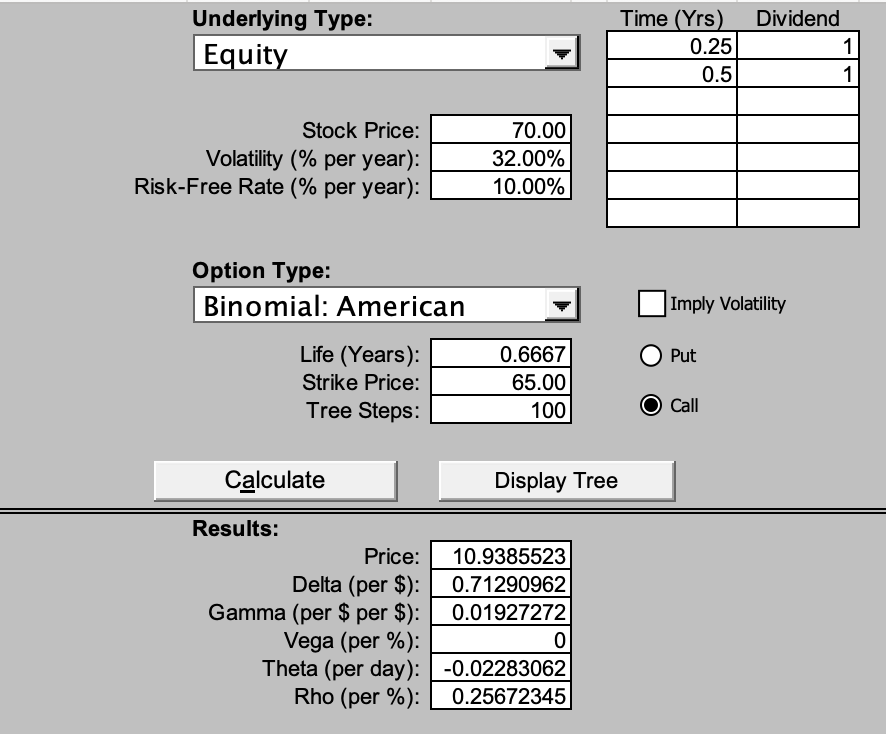
\includegraphics[width=400pt]{15_13_price.png}
\end{figure} \\ \\ \\ \\
We find the price to be approximately \boxed{\textbf{\$10.94}}.

}
{\Large 

\section*{15.15}
With the notation used in this chapter

\subsection*{(a)}
What is \(N'(x)\)? \\ \\


\subsection*{(b)}
Show that \(SN'(d_1) = Ke^{-r(T-t)}N'(d_2)\), where \(S\) is the stock price at time \(t\) 
\[
  d_1 = \frac{\ln(S / K) + (r + \sigma^2 / 2)(T - t)}{\sigma \sqrt{T - t}}
\]
\[
  d_2 = \frac{\ln(S / K) + (r - \sigma^2 / 2)(T - t)}{\sigma \sqrt{T - t}}
\] 


\subsection*{(c)}
Calculate \(\partial d_1 / \partial S\) and \(\partial d_2 / \partial S\). \\ \\


\subsection*{(d)}
Show that when 
\[
  c = SN(d_1) - Ke^{-r(T-t)} N(d_2)
\]
\[
  \frac{\partial c}{\partial d} = -r Ke^{-r(T - t)}N(d_2) - SN'(d_1) \frac{\sigma}{2 \sqrt{T - t}}
\]


\subsection*{(e)}
Show that \(\partial c / \partial S = N(d_1)\). \\ \\


\subsection*{(f)}
Show that the \(c\) satisfies the Black-Scholes-Merton differential equation. \\ \\


\subsection*{(g)}
Show that \(c\) satisfies the boundary condition for a European call option, i.e., that \(c = \max(S - K, 0)\) as \(t\) tends to \(T\). \\ \\


}
{\Large 

\section*{15.26}
Suppose that observations on a stock price (in dollars) at the end of each of 15 consecutive weeks are as follows: \\
30.2, 32.0, 31.1, 30.1, 30.2, 30.3, 30.6, 33.0, 32.9, 33.0, 33.5, 33.5, 33.7, 33.5, 33.2 \\
Estimate the stock price volatility. What is the standard error of your estimate? \\ \\


}

\end{document}